\documentclass[12pt,letterpaper]{article}
\usepackage{graphicx,textcomp}
\usepackage{natbib}
\usepackage{setspace}
\usepackage{fullpage}
\usepackage{color}
\usepackage[reqno]{amsmath}
\usepackage{amsthm}
\usepackage{fancyvrb}
\usepackage{amssymb,enumerate}
\usepackage[all]{xy}
\usepackage{endnotes}
\usepackage{lscape}
\newtheorem{com}{Comment}
\usepackage{float}
\usepackage{hyperref}
\newtheorem{lem} {Lemma}
\newtheorem{prop}{Proposition}
\newtheorem{thm}{Theorem}
\newtheorem{defn}{Definition}
\newtheorem{cor}{Corollary}
\newtheorem{obs}{Observation}
\usepackage[compact]{titlesec}
\usepackage{dcolumn}
\usepackage{tikz}
\usetikzlibrary{arrows}
\usepackage{multirow}
\usepackage{xcolor}
\newcolumntype{.}{D{.}{.}{-1}}
\newcolumntype{d}[1]{D{.}{.}{#1}}
\definecolor{light-gray}{gray}{0.65}
\usepackage{url}
\usepackage{listings}
\usepackage{color}

\definecolor{codegreen}{rgb}{0,0.6,0}
\definecolor{codegray}{rgb}{0.5,0.5,0.5}
\definecolor{codepurple}{rgb}{0.58,0,0.82}
\definecolor{backcolour}{rgb}{0.95,0.95,0.92}

\lstdefinestyle{mystyle}{
	backgroundcolor=\color{backcolour},   
	commentstyle=\color{codegreen},
	keywordstyle=\color{magenta},
	numberstyle=\tiny\color{codegray},
	stringstyle=\color{codepurple},
	basicstyle=\footnotesize,
	breakatwhitespace=false,         
	breaklines=true,                 
	captionpos=b,                    
	keepspaces=true,                 
	numbers=left,                    
	numbersep=5pt,                  
	showspaces=false,                
	showstringspaces=false,
	showtabs=false,                  
	tabsize=2
}
\lstset{style=mystyle}
\newcommand{\Sref}[1]{Section~\ref{#1}}
\newtheorem{hyp}{Hypothesis}

\title{PS02 - My Answers (Quants 1)}
\date{23.10.2025}
\author{Sarah Magdihs}

\begin{document}
	\maketitle
	\section*{Question 1: Political Science}
		\vspace{.25cm}
	The following table was created using the data from a study run in a major Latin American city.\footnote{Fried, Lagunes, and Venkataramani (2010). ``Corruption and Inequality at the Crossroad: A Multimethod Study of Bribery and Discrimination in Latin America. \textit{Latin American Research Review}. 45 (1): 76-97.} As part of the experimental treatment in the study, one employee of the research team was chosen to make illegal left turns across traffic to draw the attention of the police officers on shift. Two employee drivers were upper class, two were lower class drivers, and the identity of the driver was randomly assigned per encounter. The researchers were interested in whether officers were more or less likely to solicit a bribe from drivers depending on their class (officers use phrases like, ``We can solve this the easy way'' to draw a bribe). The table below shows the resulting data.

\begin{table}[h!]
	\centering
	\begin{tabular}{l | c c c }
		& Not Stopped & Bribe requested & Stopped/given warning \\
		\\[-1.8ex] 
		\hline \\[-1.8ex]
		Upper class & 14 & 6 & 7 \\
		Lower class & 7 & 7 & 1 \\
		\hline
	\end{tabular}
\end{table}
\newpage
\begin{enumerate}
	
	\item [(a)]
	Calculate the $\chi^2$ test statistic by hand/manually (even better if you can do "by hand" in \texttt{R}).\\
		
	\noindent{\texttt{Answer:}} 
	
	\noindent {Okay, before we can start, we need to actually 'import' this table into RStudio. So let's create our dataframe: } 
	\vspace{.25cm}
	\noindent{\texttt{R Code:}} 
	\lstinputlisting[language=R, firstline=49, lastline=63]{PS02_answersSM.R}  
	\noindent \textit{Please note: I tried several options of how to effectively create this contingency table. Since Option A has a more suitable name, we will continue with this one.}
	
	\noindent {Now, let's start with the actual task. 
	
	 There is a very simple option: R can run a $Chi^2$  test. This creates a dataframe that actually stores a lot of useful information, including the (standardised) residuals.
	 } 
	 
	 \vspace{.25cm}
	 \noindent{\texttt{R Code:}} 
	 \lstinputlisting[language=R, firstline=75, lastline=76]{PS02_answersSM.R}  
	\begin{verbatim}
		Warning message:
		In chisq.test(df) : Chi-squared approximation may be incorrect
		
		Pearson's Chi-squared test
		data:  df
		X-squared = 3.7912, df = 2, p-value =
		0.1502
	\end{verbatim}
	
	 \noindent {So , the $Chi^2$ statistic is 3.7912. Moreover, R tells us that it used two degrees of freedom. This is because the $df = (row - 1) * (column - 1)$. Moreover, it also gives us a p-value, which we will return to in a subsequent task. 
	 	
	 	Importantly, in the console, we also see that R warns us that the approximation may be incorrect. This is because one of the cells contains a value smaller than 5. 
	 } 
\vspace{.25cm}

 \noindent {Additionally, we can calculate this "by hand". Let's use the dataframe from before. Importantly, the $Chi^2$ is calculated like this: $\sum(\frac{(f_{observed}-f_{expected})^2} {f_{expected}})$. Thus, we also need to calculate the expected values for each cell. To do this, we calculate: $f_{expected}=\frac{row\:total*column\:total}{grand\:total}$, for each cell. 
 	
 	The following code shows that entire process, culminating in the $Chi^2$
} 

\noindent{\texttt{R Code:}} 
\lstinputlisting[language=R, firstline=98, lastline=131]{PS02_answersSM.R}  
\begin{verbatim}
	> chi_sq_by_hand
	[1] 3.791168
	
	> chi_square_by_R
	Pearson's Chi-squared test
	data:  df
	X-squared = 3.7912, df = 2, p-value =
	0.1502
\end{verbatim}

	
	\item [(b)]
	Now calculate the p-value from the test statistic you just created (in \texttt{R}).\footnote{Remember frequency should be $>$ 5 for all cells, but let's calculate the p-value here anyway.}  What do you conclude if $\alpha = 0.1$?\\
	\noindent{\texttt{Answer:}} 
	\noindent {Okay, let's return to the p-value that we got from R when we ran the $Chi^2$ test: 
	R shows us a p-value of roughly 0.15. Since 0.15 is bigger than 0.1, we fail to reject the $H_0$ that the two variables are independent. There is not sufficient evidence based on our sample to accept the alternative Hypothesis that they are dependent. 
	
	Once again, we can also do this "by hand". For this, we need the degrees of freedom, which, as mentioned above, are calculated as follows: $df = (row - 1) * (column - 1)$. We then compare our TS to a critical value on the $Chi^2$ distribution.} 
	
	\vspace{.25cm}
	\noindent{\texttt{R Code:}} 
	\lstinputlisting[language=R, firstline=134, lastline=146]{PS02_answersSM.R}  
	
	\begin{verbatim}
		> p_value_chi_sq
		[1] 0.1502306
	\end{verbatim}
	\newpage
	\item [(c)] Calculate the standardized residuals for each cell and put them in the table below.
	\noindent{\texttt{Answer:}} 
	
	\noindent {Okay, as mentioned before, the dataframe produced by R gives us a lot of useful info. This includes the standardised residuals.}
	\vspace{.25cm}
	
	\noindent{\texttt{R Code:}} 
	\lstinputlisting[language=R, firstline=75, lastline=76]{PS02_answersSM.R}  
		\begin{verbatim}
		> print(std_residuals_by_R)
		Not Stopped Bribe requested Stopped/given warning
		upper class   0.3220306       -1.641957              1.523026
		lower class  -0.3220306        1.641957             -1.523026
	\end{verbatim}
		\noindent{\texttt{Now, let's insert them:}} 
	\begin{table}[h]
		\centering
		\begin{tabular}{l | c c c }
			& Not Stopped & Bribe requested & Stopped/given warning \\
			\\[-1.8ex] 
			\hline \\[-1.8ex]
			Upper class  & 0.322 & -1.642 & 1.523 \\
			\\[-1.8ex]
			Lower class  & -0.322 & 1.642 & -1.523 \\
		\end{tabular}
		\caption{Standardized residuals by class and outcome}
		\label{tab:stdresiduals}
	\end{table}

	\item [(d)] How might the standardized residuals help you interpret the results?
	
	  \noindent{\texttt{Answer:}} 
	  
	\noindent {The standardized residuals can help us identify which cells or groups drive the overall difference observed in the data.  
	Cells with larger standardized residuals contribute more heavily to the $\chi^2$ statistic. If the residual is positive, it means this outcome was observed more often than expected under the Nullhypothesis. Conversely, if the residuals are negative, we actually observed a certain outcome less often than expected under the Null.}
	
	
	
\end{enumerate}
\newpage

\section*{Question 2: Economics}
Chattopadhyay and Duflo were interested in whether women promote different policies than men.\footnote{Chattopadhyay and Duflo. (2004). ``Women as Policy Makers: Evidence from a Randomized Policy Experiment in India. \textit{Econometrica}. 72 (5), 1409-1443.} Answering this question with observational data is pretty difficult due to potential confounding problems (e.g. the districts that choose female politicians are likely to systematically differ in other aspects too). Hence, they exploit a randomized policy experiment in India, where since the mid-1990s, $\frac{1}{3}$ of village council heads have been randomly reserved for women. A subset of the data from West Bengal can be found at the following link: \url{https://raw.githubusercontent.com/kosukeimai/qss/master/PREDICTION/women.csv}\\

\noindent Each observation in the data set represents a village and there are two villages associated with one GP (i.e. a level of government is called "GP"). Figure~\ref{fig:women_desc} below shows the names and descriptions of the variables in the dataset. The authors hypothesize that female politicians are more likely to support policies female voters want. Researchers found that more women complain about the quality of drinking water than men. You need to estimate the effect of the reservation policy on the number of new or repaired drinking water facilities in the villages.
\vspace{.5cm}
\begin{figure}[h!]
	\caption{\footnotesize{Names and description of variables from Chattopadhyay and Duflo (2004).}}
	\vspace{.5cm}
	\centering
	\label{fig:women_desc}
	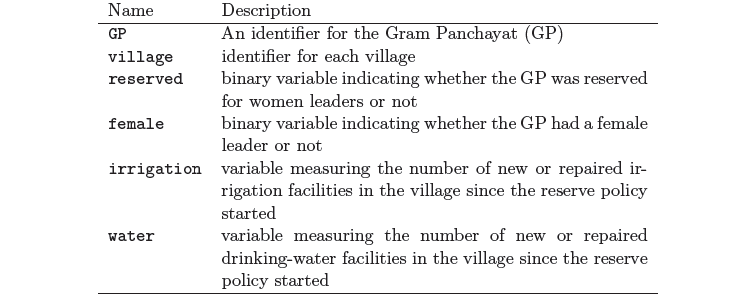
\includegraphics[width=1.1\textwidth]{women_desc.png}
\end{figure}		

\newpage
\begin{enumerate}
	\item [(a)] State a null and alternative (two-tailed) hypothesis. 
	 \noindent{\texttt{Answer:}} 
	
	\noindent {So, as stated above, we need to estimate the effect of the reservation policy on the number of new or repaired drinking water facilities in the villages.
		
	Thus, plainly speaking, the $H_0$ is that the reservation policy has \textit{no} impact on the number of new or repaired drinking water facilities in the villages. This corresponds to $H_0: \beta_1 = 0$. 
	
	The $H_a$ is that the reservation policy does have an impact on the number of new or repaired drinking water facilities in the villages. This corresponds to $H_a: \beta_1 \neq 0$. 
	\textit{Technically, given the description, the hypothesis would be that it has a positive effect, but it is a two-tailed hypothesis test, so it is AN effect.}}
	
	\item [(b)] Run a bivariate regression to test this hypothesis in \texttt{R} (include your code!).

	
	\noindent {While it is a bit naive, we're just gonna run a very simple regression model, where we regress the outcome variable on our predictor.}
	\vspace{.25cm}
	
	\noindent{\texttt{R Code:}} 
	\lstinputlisting[language=R, firstline=172, lastline=174]{PS02_answersSM.R}  
		\begin{verbatim}
		> summary(reg_1)
		
		Call:
		lm(formula = data$water ~ data$reserved)
		
		Residuals:
		Min      1Q  Median      3Q     Max 
		-23.991 -14.738  -7.865   2.262 316.009 
		
		Coefficients:
		Estimate Std. Error t value Pr(>|t|)    
		(Intercept)     14.738      2.286   6.446 4.22e-10 ***
		data$reserved    9.252      3.948   2.344   0.0197 *  
		---
		Signif. codes:  
		0 ‘***’ 0.001 ‘**’ 0.01 ‘*’ 0.05 ‘.’ 0.1 ‘ ’ 1
		
		Residual standard error: 33.45 on 320 degrees of freedom
		Multiple R-squared:  0.01688,	Adjusted R-squared:  0.0138 
		F-statistic: 5.493 on 1 and 320 DF,  p-value: 0.0197
	\end{verbatim}
	
	\vspace{6cm}
	\item [(c)] Interpret the coefficient estimate for reservation policy.
	
	 \noindent{\texttt{Answer:}} 
	 
	 \noindent {Okay, as a last step, let's interpret the output of this regression.
	 
	 The slope coefficient in a model is the (average) expected change in the outcome variable for a one-unit increase in the predictor. In this case, the predictor is binary.
	 
	 Our regression shows that based on our sample there is evidence that the reservation policy has an effect on the number of new or repaired drinking water facilities in villages (thus, we reject $H_0: \beta_1 = 0$). Specifically, we find that, on average, villages with reserved seats for women have 9.25 more new or repaired drinking water facilities than villages without such a policy.
	 
	 The intercept ($\beta_0 = 14.74$) tells us that in villages without a reservation policy, the expected number of new or repaired drinking water facilities is roughly 15.
	 
	 It is important to note that $\beta_1$ is an estimator with its own sampling distribution. Based on our sample, we can calculate a 95$\%$ confidence interval to make the uncertainty around this estimate more apparent:} 
	 
	 \noindent{\texttt{R Code:}} 
	 \lstinputlisting[language=R, firstline=183, lastline=183]{PS02_answersSM.R}  
	 	\begin{verbatim}
	 	> confint(reg_1, level =0.95)
	 	2.5 %   97.5 %
	 	(Intercept)   10.240240 19.23640
	 	data$reserved  1.485608 17.01924
	 \end{verbatim}
	 
	  \noindent {The resulting 95$\%$  confidence interval is approximately [1.49, 17.02], meaning we are 95 $\%$ confident that the true effect of the reservation policy on water infrastructure lies within this range. Since the interval does not include zero, the effect is statistically significant at the level p = 0.05
	  	
	  Hence, we conclude that the presence of reserved seats for women is associated with an increase in the number of new or repaired drinking water facilities in villages.} 
	 \vspace{.25cm}
\end{enumerate}

%\newpage
%	\section*{Question 3 (30 points): Biology}
%
%There is a physiological cost of reproduction for fruit flies, such that it reduces the lifespan of female fruit flies.  Is there a similar cost to male fruit flies?  This dataset contains observations from five groups of 25 male fruit flies. The experiment tests if increased reproduction reduces longevity for male fruit flies. The five groups are: males forced to live alone, males assigned to live with one or eight newly pregnant females (non-receptive females), and males assigned to live with one or eight virgin females (interested females). The name of the data set is \texttt{fruitfly.csv}.\footnote{Partridge and Farquhar (1981).``Sexual Activity and the Lifespan of Male Fruitflies''. \textit{Nature}. 294, 580-581.}
%	\vspace{1cm}
%
%\begin{tabular}{r|l}
%	\texttt{No} & serial number (1-25) within each group of 25\\
%	\texttt{type} & Type of experimental assignment \\
%	& \hspace{0.1in} $1=$ no females  \\
%	& \hspace{0.1in} $2=$ 1 newly pregnant female \\
%	& \hspace{0.1in} $3=$ 8 newly pregnant females\\
%	& \hspace{0.1in} $4=$ 1 virgin female\\
%	& \hspace{0.1in} $5=$ 8 virgin females\\
%	\texttt{lifespan} & lifespan (days)\\
%	\texttt{thorax} & length of thorax (mm)\\
%	\texttt{sleep} & percentage of each day spent sleeping\\
%\end{tabular}
%	\vspace{1cm}
%\begin{enumerate}
%	
%	\item
%	Import the data set and obtain summary statistiscs and examine the distribution of the overall lifespan of the fruitflies.  
%
%\newpage
%	\item
%	Plot \texttt{lifespan} vs \texttt{thorax}. Does it look like there is a linear relationship? Provide the plot. What is the correlation coefficient between these two variables?
%		\vspace{6cm}
%	\item
%	Regress \texttt{lifespan} on \texttt{thorax}.  Interpret the slope of the fitted model.
%			\vspace{6cm}
%	\item
%	Test for a significant linear relationship between  \texttt{lifespan} and \texttt{thorax}. Provide and interpret your results of your test.
%	
%\newpage
%	\item
%	
%	Provide the 90\% confidence interval for the slope of the fitted model.
%	
%			\vspace{.5cm}
%	\begin{itemize}
%		\item
%		Use the formula of confidence interval.		\vspace{.5cm}
%		\item
%		Use the function  \texttt{confint()}  in \texttt{R} .
%	\end{itemize}
%			\vspace{6cm}
%	\item Use the \texttt{predict()} function in \texttt{R} to (1) predict an individual fruitfly's lifespan when \texttt{thorax}=0.8 and (2) the average \texttt{lifespan} of fruitflies when \texttt{thorax}=0.8 by the fitted model. This requires that you compute prediction and confidence intervals. What are the expected values of lifespan? What are the prediction and confidence intervals around the expected values? 
%	
%			\vspace{6cm}
%	\item	For a sequence of \texttt{thorax} values, draw a plot with their fitted values for \texttt{lifespan}, as well as the prediction intervals and confidence intervals.
%


%\end{enumerate}
\end{document}
